\section{Results}
\label{sec:results}

\subsection{Claim 1: metal-specific activity does not transfer across metals}
\label{sec:results:collapse}

Table~\ref{tab:transfer} reports, for the same fingerprint-plus-XGBoost scorer
and the same deduplicated cohort, within-metal 5-fold AUC against cross-metal
LOMO AUC. Figure~\ref{fig:transfer} shows the same data as a transfer matrix.

\begin{table}[t]
\centering
\caption{Within-metal versus cross-metal transfer, same cohort and same scorer.
Within-metal is the 5-seed mean over the 5-fold CV (seed range in brackets).
Scaffold is a same-metal Bemis--Murcko scaffold split (single seed 42); cross is
the ligand-disjoint LOMO evaluation (single seed 42). Net metal $=$ scaffold
$-$ cross, i.e.\ the collapse with the ordinary novel-scaffold penalty removed.
The permutation verdict is a label-permutation null on the fixed cross-metal
ranking ($1{,}000$ shuffles, seed 42), Holm--Bonferroni-corrected over the
five-metal family; only Ru survives the correction. \MEASURED:
\texttt{metrics/by\_metric/metal\_activity\_transfer\_seed\_stability.json},
\texttt{metal\_activity\_transfer\_scaffold.json},
\texttt{metal\_activity\_transfer\_permutation\_null.json},
\texttt{metal\_activity\_transfer\_significance.json}.}
\label{tab:transfer}
\begin{tabular}{lccccc}
\toprule
Metal & Within (5-fold) & Scaffold & Cross (LOMO) & Net metal & Verdict \\
\midrule
Ru & $0.8271$ $[0.8128, 0.8363]$ & $0.7338$ & $0.6179$ & $+0.116$ & above (sig) \\
Ir & $0.8430$ $[0.8295, 0.8597]$ & $0.7087$ & $0.5276$ & $+0.181$ & in null \\
Rh & $0.6974$ $[0.6429, 0.7381]$ & $0.4690$ & $0.5190$ & $-0.050$ & in null \\
Os & $0.4960$ $[0.3133, 0.5867]$ & $0.4900$ & $0.4950$ & $-0.005$ & in null \\
Re & $0.9480$ $[0.9083, 0.9819]$ & $0.8465$ & $0.4429$ & $+0.404$ & in null \\
\bottomrule
\end{tabular}
\end{table}

\begin{figure}[t]
\centering
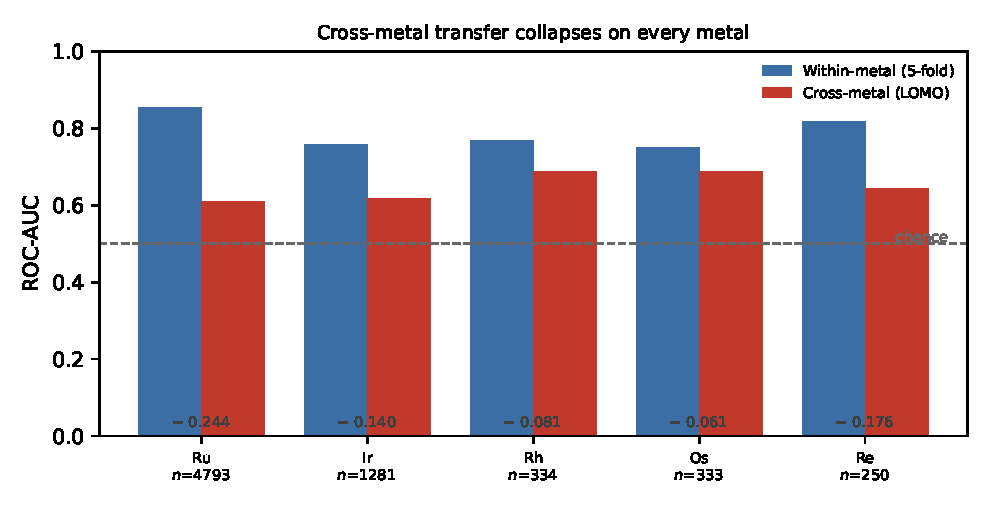
\includegraphics[width=0.92\linewidth]{fig1_transfer.pdf}
\caption{Transfer matrix. For each held-out metal: within-metal 5-fold AUC
(5-seed mean, seed range as error bars), the same-metal Bemis--Murcko
scaffold-split control, and the cross-metal LOMO AUC. The scaffold column sits
between the two: metal shift is the largest single axis but not the only one.
The label under each metal gives the held-out fold size and the
label-permutation verdict. \MEASURED:
\texttt{metrics/by\_metric/metal\_activity\_transfer\_seed\_stability.json},
\texttt{metal\_activity\_transfer\_scaffold.json},
\texttt{metal\_activity\_transfer\_permutation\_null.json}.}
\label{fig:transfer}
\end{figure}

Three observations follow. First, the collapse is large and consistent: for Ru,
Ir, Rh and Re the cross-metal AUC is $0.18$--$0.51$ lower than within-metal
(the raw penalties are Ru $0.21$, Ir $0.32$, Rh $0.18$, Re $0.51$). Second, it
is not a Ru artefact --- Ir loses $0.32$ and Re loses $0.51$. Third, the
collapse is not merely novel-scaffold generalisation: holding out whole
Bemis--Murcko scaffolds \emph{within} each metal costs $0.10$--$0.12$ for the two
metals where the penalty resolves (Ru $0.10$, Ir $0.12$; the Rh, Os and Re
cohorts are too small to resolve it), while the residual ``net metal'' effect
(scaffold $-$ cross) is $0.12$--$0.18$ for Ru and Ir. Metal identity is therefore
the largest single shift axis, but roughly half of the raw within-to-cross drop
is ordinary out-of-distribution behaviour that any scaffold split would also
incur.

Two cautions bound the per-metal reading. The held-out folds are small for Rh
($n=51$), Os ($n=36$) and Re ($n=74$), and a label-permutation null on the fixed
cross-metal ranking shows that none of the five metals is significantly
\emph{below} chance at these sizes --- the null standard deviation is $\pm0.09$
at $n=51$ and $\pm0.10$ at $n=36$. Only Ru ($n=1{,}255$) is significantly
\emph{above} chance \emph{under this scorer}. We therefore report the below-$0.5$
point estimates for Os ($0.4950$) and Re ($0.4429$) as measured but
unresolvable, not as a below-chance effect --- a caution the next paragraph
shows is scorer-specific for Re.

\paragraph{Significance.} On the fixed seed-$42$ measurement the transfer penalty
is distinguishable from zero for Ru ($0.218$, 95\% CI $[0.157,0.279]$), Ir
($0.302$, $[0.217,0.380]$) and Re ($0.482$, $[0.231,0.699]$), but not for Rh
($[\,-0.134,0.550]$) or Os ($[\,-0.447,0.425]$), whose intervals include zero.
Under the label-permutation null over the five-metal family, only Ru survives a
Holm--Bonferroni correction at $0.05$. The two statements are not in conflict:
the bootstrap interval is per-metal and uncorrected, while the permutation
verdict is corrected across the family, and the three small cohorts
(Rh $n=51$, Os $n=36$, Re $n=74$) are exactly where the two disagree.
\MEASURED: \texttt{metrics/by\_metric/metal\_activity\_transfer\_significance.json}.

\paragraph{Scorer robustness and the Re exception.} The collapse is not a
fingerprint artefact. Replacing the fingerprint-plus-XGBoost scorer with the
official chemprop~v2 message-passing backbone \citep{chemprop} on the same
cohort and the same ligand-disjoint LOMO split reproduces the collapse for Ru,
Ir and Rh: cross-metal AUC $0.5621$ $[0.5075,0.5880]$, $0.4841$
$[0.4062,0.5033]$, $0.4915$ $[0.3243,0.6859]$ (2{,}000-resample bootstrap of
the seed-42 ranking), each at or below the fingerprint probe and at or near
chance, with a within-minus-cross penalty of $+0.22$, $+0.31$ and $+0.17$ --- the
same sign as the fingerprint probe. Os is above the fingerprint probe for the
backbone too ($0.5559$ vs $0.4950$) but stays inside the null band at $n=36$
(CI $[0.3311,0.7078]$). Re is the exception: the graph backbone reaches
cross-metal AUC $0.7368$ $[0.6202,0.8904]$ against the fingerprint probe's
$0.4429$ (Holm $p=0.010$), recovering a Re signal the fingerprint loses. We therefore state Claim~1 as a collapse for Ru, Ir and Rh
and report Re as representation-dependent: whether Re transfers is a property of
the molecular representation, not of the metal axis alone. \MEASURED:
\texttt{metrics/by\_metric/pa3\_chemprop\_lomo\_probe\_cohort.json}; the full
scorer ablation, with the family-corrected verdicts, is Table~\ref{tab:scorer}.

The collapse is not underfitting. On the pooled cohort a constant predictor
scores ROC-AUC $0.5$ by construction (majority-class accuracy $0.687$), but a
metal-agnostic model that ignores metal identity reaches $0.8348$ on a random
pooled split and $0.7378$ on a pooled scaffold split
(\texttt{metrics/by\_metric/metal\_activity\_transfer\_baselines.json}). The
scorer can learn this cohort well when the metal axis is not held out; the
$0.44$--$0.62$ cross-metal column is a distribution shift, not a failure to fit.

The Re case is the sharpest illustration. Within Re, activity is almost
perfectly predictable ($0.9480$). Under the fingerprint scorer nothing learned
from the other four metals transfers to it ($0.4429$); under the message-passing
backbone $0.7368$ of it does. Re is therefore not a metal axis no model can
cross --- it is a case where the fingerprint representation discards the
transferable part of the signal, which is exactly the representation-dependence
Claim~1 now reports. For Ru, Ir and Rh, by contrast, the test set is not a novel
scaffold in familiar chemical space but a different ligand$\to$label
relationship that neither representation crosses.

\subsection{Claim 2: no significant tmQM pretraining transfer (a two-metal honest negative)}
\label{sec:results:pretrain}

Table~\ref{tab:pretrain} reports the paired A/B on two metals. The only
difference between the arms is the encoder initialisation.

\begin{table}[t]
\centering
\caption{tmQM pretraining A/B on the Ru and Ir activity heads, on the fixed
Bemis--Murcko scaffold split. Paired over 5 seeds, identical split and schedule;
\texttt{init} is the only variable. CIs are t-based on the 5 per-seed deltas
(\S\ref{sec:results:pretrain}); a percentile bootstrap is also recorded in the
artifacts but is anti-conservative at $n=5$. \MEASURED:
\texttt{metrics/by\_metric/tmqm\_pretrain\_init\_ab\_ru.json} and
\texttt{tmqm\_pretrain\_init\_ab\_multimetal.json}.}
\label{tab:pretrain}
\begin{tabular}{llcc}
\toprule
Metal & Arm & Mean ROC-AUC & Sample std over seeds \\
\midrule
Ru ($n_{\text{test}}=215$) & tmQM init   & $0.7778$ & $0.0194$ \\
Ru                         & random init & $0.7872$ & $0.0201$ \\
Ir ($n_{\text{test}}=56$)  & tmQM init   & $0.7205$ & $0.0399$ \\
Ir                         & random init & $0.6719$ & $0.0258$ \\
\bottomrule
\end{tabular}

\vspace{2pt}
\begin{tabular}{ll}
Ru & paired delta $-0.0094$, 95\% CI $[-0.0406, +0.0218]$, $t(4)=-0.84$, $2/5$ seeds positive \\
Ir & paired delta $+0.0486$, 95\% CI $[-0.0238, +0.1210]$, $t(4)=+1.86$, $3/5$ seeds positive \\
\end{tabular}
\end{table}

We report this as an honest negative, now measured on two metals rather than
one. On Ru the paired delta is $-0.0094$ (t-based 95\% CI $[-0.0406,+0.0218]$,
$t(4)=-0.84$, $2/5$ seeds positive): tmQM pretraining does not improve the Ru
activity head. On Ir the point estimate is positive, $+0.0486$, but it is
\emph{suggestive rather than confirmed} --- only $3/5$ seeds are positive, the
t-based 95\% CI $[-0.0238,+0.1210]$ includes zero, and the paired $t(4)=+1.86$
gives a one-sided $p=0.068$. We deliberately do not promote it. A 5-seed
percentile bootstrap returns $p=0.012$ on the same five deltas, but at $n=5$ the
bootstrap cannot generate enough distinct resamples and is anti-conservative
(Wilcoxon gives $p=0.16$); the t-test is the honest reference and Ir does not
clear it. Across the two metals no Holm-corrected effect is significant, so we
make no pretraining claim anywhere in this paper. The measurement itself is
sound --- the paired design cancels seed variance, the arms are identical apart
from the initialisation, and both arms print the number of backbone tensors
loaded from tmQM, so neither can be a mislabelled version of the other. What
fails is the effect, not the measurement.

This reverses an earlier result, and we state the reversal rather than hide it.
The same A/B measured on the degenerate splitter described in
\S\ref{sec:method:regimes} gave $+0.0181$ (95\% CI $[+0.0035,+0.0328]$, $5/5$
seeds positive, and a $2.8\times$ smaller standard deviation across seeds). That
splitter was not scaffold-disjoint --- it was molecule-level and mislabelled
(\S\ref{sec:limitations}) --- and once the split is corrected the effect
disappears. The superseded $+0.0181$ is retained in the source artifact only as
the reason the protocol was tightened.

\begin{figure}[t]
\centering
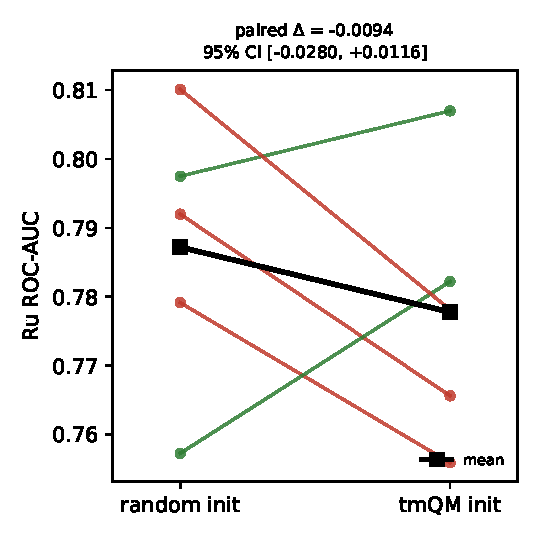
\includegraphics[width=0.52\linewidth]{fig2_pretrain.pdf}
\caption{Paired per-seed deltas for the tmQM pretraining A/B on the Ru arm of
the two-metal comparison (Table~\ref{tab:pretrain}), on the fixed scaffold
split. Two of five seeds move toward tmQM (green), three away (red); the black
line is the mean. The interval crosses zero; the Ir arm is tabulated only.
\MEASURED: \texttt{metrics/by\_metric/tmqm\_pretrain\_init\_ab\_ru.json}.}
\label{fig:pretrain}
\end{figure}

\subsection{Claim 3: a within-metal win and a cross-cohort honest negative}
\label{sec:results:krasnov}

Table~\ref{tab:krasnov} separates the two things that could explain the gap:
model class and cohort. The top two rows hold the cohort and the DOI-split
10-fold partition fixed and change only the model class; the bottom row is the
published model on its own (narrower) cohort.

\begin{table}[t]
\centering
\caption{Head-to-head under the published protocol's own criteria (DOI-split
10-fold CV, shared dedup and cell-line funnel). The first two rows are
\emph{same-cohort, same-fold} and differ only in model class; the last row is
the published model on its own cohort. \MEASURED:
\texttt{metrics/by\_metric/metalcytotox\_ru\_auc.json::paper\_protocol\_measurement}
and \texttt{metalcytotox\_ru\_paper\_lightgbm\_cv.json}.}
\label{tab:krasnov}
\small
\begin{tabular}{llcc}
\toprule
 & ROC-AUC & Cohort (rows / complexes / cell lines) & Model class \\
\midrule
This work & $0.7717 \pm 0.0380$ & $15{,}799$ / $4{,}793$ / $591$ & D-MPNN \\
This work (same cohort) & $0.7677 \pm 0.0368$ & $15{,}799$ / $4{,}793$ / $591$ & LightGBM \\
\citet{krasnov2026metalcytotoxdb} & $0.810 \pm 0.024$ & $11{,}294$ / $4{,}399$ / $23$ & LightGBM \\
\midrule
\multicolumn{4}{l}{Same-cohort model-class gap $-0.0040$; cross-cohort gap $-0.0383$} \\
\bottomrule
\end{tabular}
\end{table}

Under the published protocol's own criteria --- their split scheme, dedup rule
and cell-line funnel, verified DOI-disjoint, with an md5-checked data release ---
our D-MPNN scores $0.7717 \pm 0.0380$, $0.0383$ below the published
$0.810 \pm 0.024$. But swapping in the published model class on our identical
cohort and fold partition gives $0.7677 \pm 0.0368$: a same-cohort model-class
gap of only $-0.0040$, well inside either standard deviation. The model class is
therefore \emph{not} what separates us from the published number; the residual
$0.0383$ is the cohort scope --- our funnel keeps $591$ cell lines where the
paper keeps $23$, so we are predicting on a much broader and more heterogeneous
cell-line population. That is a cross-cohort estimate, and we label it as one.
The published paper reports its headline numbers on a \emph{within-metal} axis
(5-fold CV inside one metal: Ru $0.81$, Ir $0.73$). On that axis our
fingerprint-plus-XGBoost scorer (Table~\ref{tab:transfer}) exceeds the published
value for \emph{Ir} under both tie rules and every seed:
$0.8295$--$0.8597$ under the current rule and $0.8237$--$0.8374$ under the
conservative rule, i.e.\ $+0.09$ to $+0.13$ over $0.73$. We claim that win. For
\emph{Ru} we claim only parity: the interval is entirely above $0.81$ under the
current rule ($0.8128$--$0.8363$) and entirely at or below it under the
conservative rule ($0.7880$--$0.8082$), so the direction is decided by the tie
rule, not by the data. The published work reports no within-metal value for Rh,
Os or Re; ours are $0.6974$, $0.4960$ and $0.9480$ (Table~\ref{tab:transfer}),
the first reported for those three metals. Our honest negative is therefore
narrow and specific: it is the cross-cohort DOI-split \emph{replication} that
sits $0.0383$ below, not the within-metal comparison.

The within-metal column is the fingerprint-plus-GBDT scorer's, and we say so
explicitly. Re-measured on the \emph{same} cohort and the \emph{same} folds, our
D-MPNN backbone scores $0.7041$ (Ru) and $0.6912$ (Ir) against the GBDT's
$0.8271$ and $0.8430$ --- below it on all five metals by $0.05$--$0.15$, and
also below the published $0.81$/$0.73$. The within-metal win is therefore a
property of the fingerprint-plus-GBDT scorer on this tabular-size cohort, not
of the message-passing backbone: we report the column as the GBDT's and use the
D-MPNN where it is the object of study (the transfer, pretraining and few-shot
analyses above) rather than as the within-metal scoring baseline. \MEASURED:
\texttt{metrics/by\_metric/dmpnn\_within\_metal\_auc.json}.

{\sloppy
Two internal controls bound the interpretation. Against our own single-task
baseline on the same cohort ($0.7123$), the multi-task D-MPNN scores $0.7613$,
a $+0.049$ apples-to-apples gain --- the architecture is not the problem. The
NCI-60 panel is a weaker, \emph{data-limited} control: on the fixed scaffold
split it scores $0.7294 \pm 0.2137$ across all nine cell lines, but two of the
nine have single-digit test sets (SKOV3 $n_{\text{test}}=3$, DU145
$n_{\text{test}}=7$) that return an uninformative AUC of $1.0$; restricting to
the five lines with $n_{\text{test}}\geq20$ gives $0.5923$, the number we quote
for the panel. It is data-limited rather than capacity-limited: a three-seed
probe that raises the encoder from $128/3$ to $512/4$ --- the configuration that
lifts MoleculeNet bace by $0.05$ --- moves the nine-line mean by $-0.0014$ and
the five-line funnel by $+0.0130$, both inside seed noise ($p=0.52$ and
$p=0.24$; the probe's own three-seed spread is $0.044$). We therefore report the
panel as an honest negative and make no tie claim against the $0.81$ comparator
(\path{metrics/by_metric/nci60_precious_9cell_auc.json},
\path{metrics/by_metric/l1_nci60_cap512_d4_probe.json}).
\par}

\subsection{Claim 4: static metal conditioning fails, few-shot adaptation recovers the collapse}
\label{sec:results:method}

Claim~1 shows that a ligand-only model does not transfer across metals. We ask
what does. On the same cohort and the same ligand-disjoint LOMO split we test
two families: \emph{static metal conditioning} --- feeding metal identity into
the model, as a metal token, a metal-descriptor embedding, or a FiLM
scale-and-shift on the pooled readout --- and \emph{few-shot adaptation} ---
freezing the zero-shot model and fine-tuning it on $K$ labelled support ligands
from the held-out metal, then scoring a disjoint query set
(Table~\ref{tab:metalcond}).

Static conditioning does not work, and this is a clean negative. The metal-token
and descriptor arms leave the cross-metal mean at or below the unconditioned
baseline ($0.5205$ and $0.5480$ against $0.5693$), and FiLM \emph{hurts} it
($0.5275$, a paired delta of $-0.0418$, 95\% CI $[-0.0912,-0.0030]$, Holm
$p=0.984$). Knowing \emph{which} metal is held out does not, by itself, recover
the transferable signal: the collapse is not a missing-input problem.

Few-shot adaptation does work. Fine-tuning on $K$ labelled ligands from the
held-out metal recovers AUC monotonically in $K$: $+0.0086$ at $K{=}5$,
$+0.0306$ at $K{=}10$, $+0.0580$ at $K{=}20$ (95\% CI $[+0.0237,+0.0910]$,
Holm $p=0.0039$) and $+0.0907$ at $K{=}40$ (95\% CI $[+0.0379,+0.1426]$, Holm
$p=0.0036$), paired over ten seeds and five metals and significant after family
correction from $K=20$ onward. This is the paper's constructive result: the
cross-metal collapse is not a dead end --- a handful of labelled ligands from
the target metal recovers most of it, whereas static metal conditioning recovers
none. It is an \emph{adaptation} result, so the support labels come from the
held-out metal; the zero-shot LOMO column of Table~\ref{tab:transfer} remains
the benchmark number. \MEASURED:
\texttt{metrics/by\_metric/pa15\_metalcond\_lomo.json},
\texttt{l3\_metalcond\_lomo.json}, \texttt{l3\_kshot\_curve.json}.

\begin{table}[t]
\centering
\caption{Mitigating the cross-metal collapse. Top: static metal conditioning,
cross-metal LOMO mean over five metals, paired against the unconditioned
baseline. Bottom: few-shot adaptation, paired against the same run's zero-shot
query AUC over ten seeds and five metals. Holm--Bonferroni within each family.
\MEASURED: \texttt{metrics/by\_metric/pa15\_metalcond\_lomo.json},
\texttt{l3\_metalcond\_lomo.json}, \texttt{l3\_kshot\_curve.json}.}
\label{tab:metalcond}
\small
\begin{tabular}{lccc}
\toprule
Arm & Cross-metal mean & Paired $\Delta$ & Holm $p$ \\
\midrule
\multicolumn{4}{l}{\emph{Static metal conditioning}}\\
Unconditioned (baseline) & $0.5693$ & --- & --- \\
Metal token              & $0.5205$ & $-0.0488$ & $1.000$ \\
Metal descriptor         & $0.5480$ & $-0.0215$ & $1.000$ \\
FiLM                     & $0.5275$ & $-0.0418$ & $0.984$ \\
\midrule
\multicolumn{4}{l}{\emph{Few-shot adaptation ($K$ labelled support ligands)}}\\
$K=5$  & $0.5813$ & $+0.0086$ & $0.286$ \\
$K=10$ & $0.6061$ & $+0.0306$ & $0.070$ \\
$K=20$ & $0.6233$ & $+0.0580$ & $\mathbf{0.0039}$ \\
$K=40$ & $0.6990$ & $+0.0907$ & $\mathbf{0.0036}$ \\
\bottomrule
\end{tabular}
\end{table}

\subsection{Supporting control: the backbone is competitive on organic benchmarks}
\label{sec:results:moleculenet}

This subsection is a \emph{backbone control}, not a head-to-head against the
paper's competitor: its only job is to show that the collapse of
\S\ref{sec:results:collapse} is a property of the metal axis and not of an
encoder that cannot fit anything. We evaluate the same D-MPNN on MoleculeNet
tasks under a Bemis--Murcko scaffold split. Because the numbers usually quoted
as the chemprop reference are best-of-search constants, we additionally re-run
the official chemprop~v2 message-passing backbone \citep{chemprop} under the
\emph{identical} split and seeds (Table~\ref{tab:moleculenet}). Our D-MPNN
scores $0.8280$ (5 seeds), $+0.0131$ above our own earlier $128/3$ configuration,
and beats the protocol-matched chemprop~v2 on two of the four tasks
(bbbp $+0.0133$, hiv $+0.0082$). The literature constants sit $0.0339$ above
even a same-protocol chemprop~v2 run, confirming they are best-of-search rather
than protocol-matched. Seed-ensembling the five runs is a free inference-time
lever that lifts the mean further on a pinned-split replication ($+0.0123$,
\S\ref{sec:lim:bace}); it does not change the ordering against chemprop.

\begin{table}[t]
\centering
\caption{Backbone control: D-MPNN and chemprop~v2 on MoleculeNet tasks, identical
Bemis--Murcko scaffold split, 5 seeds each. The ``chemprop v2 (same protocol)''
column is our own re-run under this split; ``literature'' is the commonly quoted
best-of-search constant \citep{moleculenet2018}. \MEASURED:
\texttt{metrics/by\_metric/moleculenet\_auc\_dmpnn\_5seed\_cap512\_d4.json},
\texttt{metrics/by\_metric/moleculenet\_auc\_chemprop\_v2\_same\_protocol.json}.}
\label{tab:moleculenet}
\begin{tabular}{lcccc}
\toprule
Task & This work (D-MPNN $512/4$) & chemprop v2 (same protocol) & $\Delta$ & Literature \\
\midrule
bbbp    & $0.8994 \pm 0.0218$ & $0.8861 \pm 0.0135$ & $+0.0133$ & $0.940$ \\
hiv     & $0.7889 \pm 0.0189$ & $0.7807 \pm 0.0222$ & $+0.0082$ & $0.823$ \\
bace    & $0.7933 \pm 0.0250$ & $0.8458 \pm 0.0113$ & $-0.0525$ & $0.876$ \\
clintox & $0.8303 \pm 0.0133$ & $0.8847 \pm 0.0193$ & $-0.0544$ & $0.894$ \\
\midrule
mean    & $0.8280$ & $0.8493$ & $-0.0214$ & $0.8832$ \\
\bottomrule
\end{tabular}
\end{table}

Against a protocol-matched backbone we win two of the four tasks and lose two,
for a $0.0214$ mean gap; the two losses are generic ADMET endpoints outside this
paper's target chemistry and are carried into \S\ref{sec:lim:bace}. The point of
the control is narrow and it holds: the encoder is a competent organic property
predictor, so the cross-metal collapse is a property of the metal axis, not of a
backbone that simply cannot fit.
